La mancata comprensione delle attività richieste nel periodo di Progettazione Architetturale, in particolare riguardanti la Technology Baseline, ha portato ad alcuni cambiamenti rispetto al prospetto orario che era stato preventivato. In particolare, le ore destinate al ruolo di \textit{Progettista} non sono state svolte in toto, poiché durante questa fase non è richiesto progettare l'applicativo in tutte le sue parti, tale attività compete al periodo successivo alla di Progettazione in Dettaglio e Codifica. Infine, come si può notare dal consuntivo, sono state necessarie più ore di quelle preventivate per i seguenti ruoli:
\begin{itemize}
	\item \RdP{}: il \Res{} ha dovuto fare da mediatore all'interno dei componenti del gruppo soprattutto durante la fase di scelta degli strumenti tecnologici;
	\item \ana{}: per la correzione e l'incremento del documenti presentati in ingresso alla Revisione dei Requisiti e in seguito al colloquio avvenuto con la Proponente;
	\item \ver{}: per la verifica dei documenti che avevano necessità di un'ulteriore verifica conseguentemente al colloquio avvenuto con la Proponente;
	\item \progr{}: le ore per la realizzazione del PoC non erano state preventivate  in quanto non si erano comprese le richieste del Committente per la Revisione di Progettazione. 
\end{itemize} 
Questo ha portato ad un incremento delle ore preventivate per persona (29 ore) rendicontando un totale di 30 ore per componente.
Malgrado l'incremento orario, le ore da \textit{Progettista} non svolte ha portato un risparmio di \euro 136,00, tale valore non scende sotto la soglia minima richiesta dal Committente ma è da tenere sotto stretto controllo, in quanto sinonimo di una scarsa comprensione delle richieste avanzate dal Committente.

\paragraph{Attività future}\mbox{}\\
In considerazione degli errori commessi, si ritiene opportuno ripianificare le attività per i periodi futuri 
relativi alla Progettazione in Dettaglio e Codifica e alla Verifica e Validazione. 


%Le regole adottate per tale ridistribuzioni sono:
%\begin{itemize}
%	\item Il non superamento delle 105 ore individuali;
%	\item Il prezzo preventivato non può superare il valore stabilito alla Revisione dei Requisiti;
%	\item La quantità di investimento deve essere tenuta strettamente sotto controllo.
%\end{itemize}
%\newpage
%Per la Progettazione in Dettaglio e Codifica il prospetto orario che si propone è il seguente: 
%
%\begin{table}[H]	
%	\begin{center}
%	    \begin{tabular}{cccccccc}
%			\rowcolor{greySWEight}
%			\textcolor{white}{\textbf{Nome}} & \textcolor{white}{\textbf{Re}} & \textcolor{white}{\textbf{Am}} & \textcolor{white}{\textbf{An}} & \textcolor{white}{\textbf{Pj}} & \textcolor{white}{\textbf{Pr}} & \textcolor{white}{\textbf{Ve}} & \textcolor{white}{\textbf{Totale}}
%			\\ 
%			Bacco Alberto & & & 8 & 12 & 12 & 20 & 52 \\
%			Caccaro Sebastiano & & 5 & 2 & 17 & 13 & 15 & 52 \\
%			Ciagola Damien & & & & 20 & 12 & 20 & 52 \\
%			Corti Francesco & 5 & 5 & & 13 & 17 & 12 & 52 \\
%			Isachi Gheorghe & & & & 14 & 20 & 18 & 52 \\
%			Legrottagle Gionata & 5 & & & 17 & 10 & 20 & 52 \\
%			Magarotto Francesco & & & & 17 & 15 & 20 & 52 \\
%			Muraro Enrico & & & & 15 & 17 & 20 & 52 \\
%			\end{tabular}
%	    \caption{Tabella della suddivisione oraria proposta per i membri del gruppo nel periodo di Pianificazione di Dettaglio e Codifica} \label{tab:tabellaPropostaPersonePianificazione di dettaglio e codifica} 
%	\end{center}
%\end{table}
%\begin{figure}[H]
%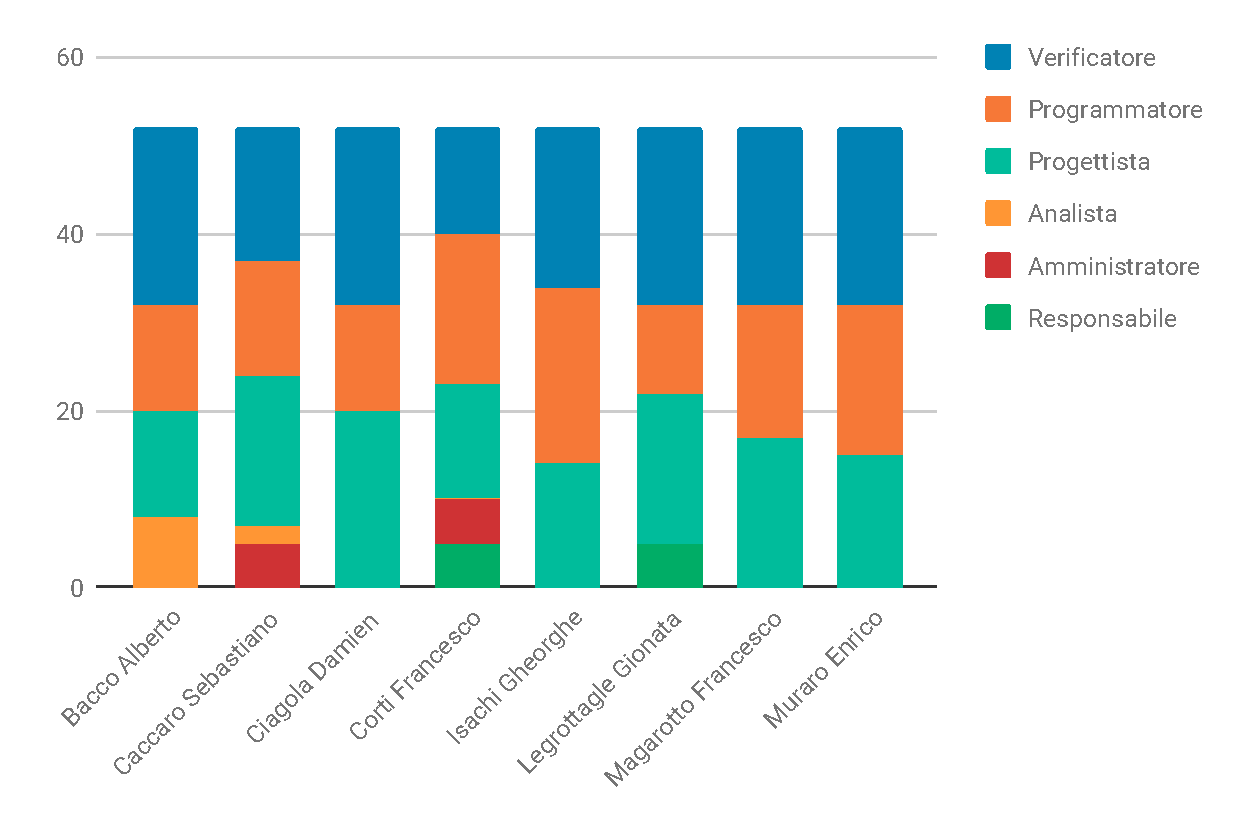
\includegraphics[width=1\linewidth]{Consuntivo/grafici/ConsPC1.pdf}
%\caption{Grafico ridistribuzione oraria per la Revisione di Qualifica proposto}
%\end{figure}
%
%Per quanto riguarda il periodo di Verifica e Validazione, il prospetto orario che viene proposto è il seguente:
%\begin{table}[H]	
%	\begin{center}
%	    \begin{tabular}{cccccccc}
%			\rowcolor{greySWEight}
%			\textcolor{white}{\textbf{Nome}} & \textcolor{white}{\textbf{Re}} & \textcolor{white}{\textbf{Am}} & \textcolor{white}{\textbf{An}} & \textcolor{white}{\textbf{Pj}} & \textcolor{white}{\textbf{Pr}} & \textcolor{white}{\textbf{Ve}} & \textcolor{white}{\textbf{Totale}}
%			\\
%			Bacco Alberto & & 5 & & & 5 & 12 & 22 \\
%			Caccaro Sebastiano & & & & & 5 & 17 & 22 \\
%			Ciagola Damien & 5 & & & & 12 & 5 & 22 \\
%			Corti Francesco & & & 5 & & & 17 & 22 \\
%			Isachi Gheorghe & 5 & & & & & 17 & 22 \\
%			Legrottagle Gionata & & & & & 10 & 12 & 22 \\
%			Magarotto Francesco & & 5 & & & 12 & 5 & 22 \\
%			Muraro Enrico & 5 & & & & & 17 & 22 \\
%			\end{tabular}
%	    \caption{Tabella della suddivisione oraria proposta per i membri del gruppo nel periodo di Verifica e Validazione} \label{tab:tabellaPropostaPersoneVerifica e validazione} 
%	\end{center}
%\end{table}
%\begin{figure}[H]
%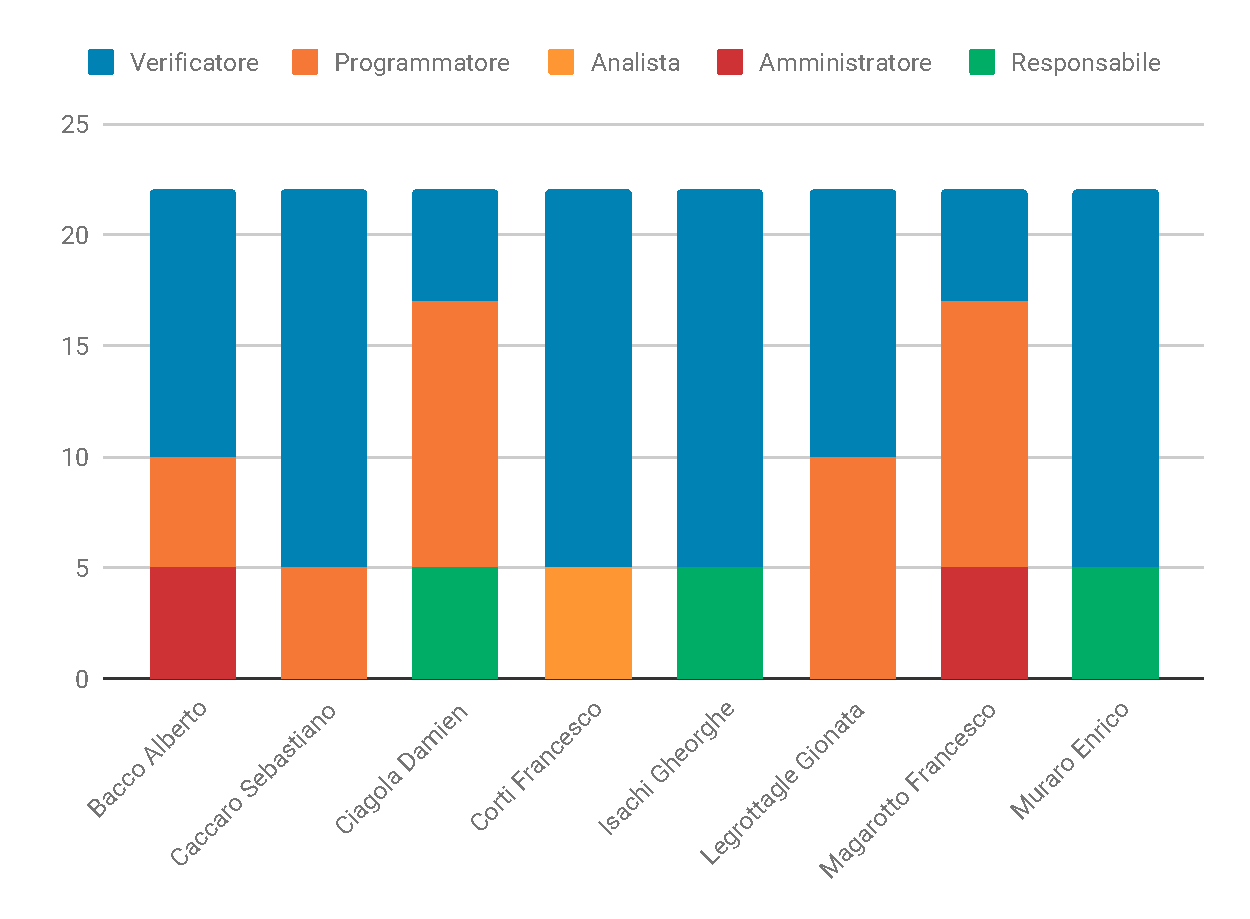
\includegraphics[width=1\linewidth]{Consuntivo/grafici/ConsVV1.pdf}
%\caption{Grafico ridistribuzione oraria per il periodo di Verifica e Validazione proposto}
%\end{figure}
Tali ridistribuzioni orarie devono lasciare invariato il costo preventivato senza modificare 
ore e ruoli dei componente del gruppo. Al contempo devono anche rispettare le seguenti direttive:
\begin{itemize}
	\item Uniformare la preparazione dei componenti. In quanto per il periodo di Progettazione in Dettaglio e Codifica per alcuni componenti non sono state preventivate ore di codifica;
	\item Permettere ad ogni componente del gruppo di svolgere almeno una volta ogni ruolo per un minimo di 5 ore durante tutto il progetto. 	
\end{itemize}
%In riferimento a quest'ultimo punto il grafico a seguire mostra le ore per componente durante il periodo rendicontato del progetto:
%\begin{figure}[H]
%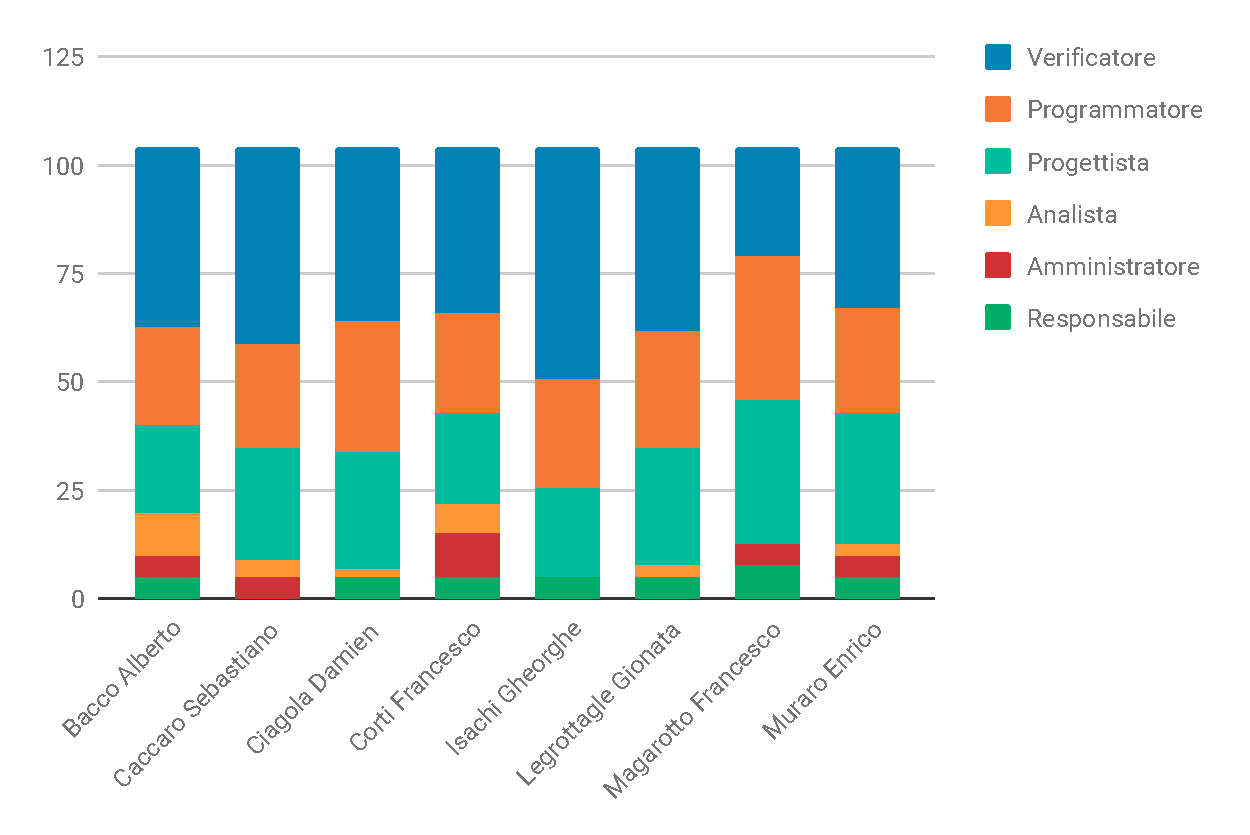
\includegraphics[width=1\linewidth]{Consuntivo/grafici/ConsTR1.pdf}
%\caption{Grafico ridistribuzione oraria reindicontata}
%\end{figure}
